% \documentclass[12pt,slidescentered,compress,serif,mathserif,professionalfont,trans,notes=show]{beamer}
\documentclass[]{beamer}

\usepackage{ucs}
\usepackage[utf8]{inputenc}
\usepackage{beamerthemeboxes}

\usepackage{amsmath}
\usepackage{amsfonts}
\usepackage{amssymb}
\usepackage{amsthm}
\usepackage{mathptmx}
\usepackage{multicol}
\usepackage{rotating}
\usepackage{xcolor}
%\usepackage[portuguese]{babel}
\usepackage[T1]{fontenc}
\usepackage{graphicx}
\usepackage{graphics}


\addtobeamertemplate{navigation symbols}{}{%
    \usebeamerfont{footline}%
    \usebeamercolor[fg]{footline}%
    \hspace{1em}%
    \insertframenumber/\inserttotalframenumber
}


\author{Leonardo Goliatt}
\title{MAC024 -- Introdução à Modelagem Computacional}
\date{}

\begin{document}
 
 \maketitle
 
\begin{frame}
\tableofcontents
\end{frame}

 

%================================================================================
\section{Apresentação}
%================================================================================

%--------------------------------------------------------------------------------
\subsection{Plano de Ensino}
%--------------------------------------------------------------------------------
%--
\begin{frame}{\insertsection}{\insertsubsection}
\begin{itemize}
\item Introdução aos sistemas dinâmicos: modelagem da mudança através de equações de diferença.
\item Classificação de Modelos, análise do processo de modelagem e construção de modelos matemáticos e sua simulação computacional.
\item Ajuste de curvas.
\item Introdução ao Método de Monte Carlo.
\item Análise Dimensional.
\end{itemize}
\end{frame}
%--
\begin{frame}{\insertsection}{\insertsubsection}
Bibliografia:

\begin{enumerate}
\item 
Giordano, F.R, Fox,W.P., Horton, S.B. e Weir, M.D., A First Course in Mathematical Modeling, Brooks Cole, 2008.
\item
Velten, K., Mathematical Modeling and Simulation, Wiley-VCH, 2009.
\item
de Vries, G., Hilen, T., Lewis, M., Müller, J. and Schönfisch, B., A Course in Mathematical Biology, SIAM, 2006.
\item
Anton,H., Rorres, C., Álgebra linear com aplicações, Bookman, 2002.
\end{enumerate}
\end{frame}
%--
\begin{frame}{\insertsection}{\insertsubsection}
Avaliações:

\begin{itemize}
 \item As avaliações ocorrerão de forma contínua ao longo do período
 \item Todas as avaliações envolvem o desenvolvimento de um modelo computacional
 \item Relatórios e apresentações em slides
\end{itemize}

Nota final:
\begin{itemize}
 \item Média das avaliações realizadas ao longo do período.
\end{itemize}

\end{frame}
%--
%--------------------------------------------------------------------------------
\subsection{Introdução}
%--------------------------------------------------------------------------------
%--
\begin{frame}{\insertsection}{\insertsubsection}
\begin{center}
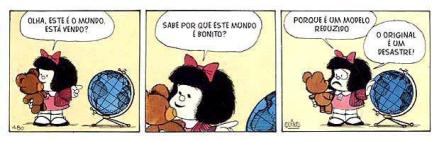
\includegraphics[width=0.8\textwidth]{./img/mafalda-e-o-mundo-desastre}
\end{center}
\end{frame}
%--
\begin{frame}{\insertsection}{\insertsubsection}
\begin{itemize}
\item O que é Modelagem Matemática?

\begin{itemize}
 \item Representação de um problema real numa forma matemática\footnote{mais abrangente possível} com hipotéses simplificadas que ajudam a entendê-lo de  uma maneira fundamental e quantitativa.
 \item Complementada com teoria e experimentos.
 \item Áreas: Ciências, Engenharias e Tecnologia, Biologia, Saúde e áreas interdisciplinares.
\end{itemize}
\end{itemize}
\end{frame}
%--
\begin{frame}{\insertsection}{\insertsubsection}
\begin{itemize}
\item Por quê a Modelagem é necessária?

\begin{itemize}
 \item Representação de um problema real numa forma matemática com hipóteses simplificadas que ajudam a entendê-lo de  uma maneira fundamental e quantitativa.
 \item Complementada com teoria e experimentos.
 \item Áreas: Ciências, Engenharias e Tecnologia, Biologia, Saúde e áreas interdisciplinares.
\end{itemize}
\end{itemize}

\end{frame}
%--
\begin{frame}{\insertsection}{\insertsubsection}

Gartner's 2016 Hype Cycle for Emerging Technologies

\begin{center}
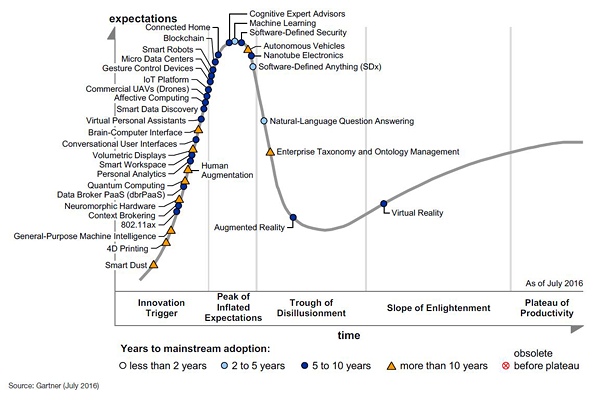
\includegraphics[width=0.99\linewidth]{./img/emerging-tech-hc-2016}
\end{center}
\end{frame}
%--
\begin{frame}{\insertsection}{\insertsubsection}
\begin{itemize}
 \item Por que um modelo matemático é necessário?
 \begin{itemize}
  \item Realizar experimentos pode ser custoso, demorado ou arriscado.
  \item Um modelo matemático emerge como uma alternativa para estudar uma variedade de problemas em pesquisa científica, produtos   e processos de manufatura.
  \item Melhora a qualidade evitando o retrabalho.
 \end{itemize}

\end{itemize}
\end{frame}
%--
\begin{frame}{\insertsection}{\insertsubsection}
\begin{itemize}
\item E Modelagem Computacional?
\begin{itemize}
\item A solução de problemas reais podem resultar em  relações matemáticas  complicadas (grande escala).
\item Há a necessidade de simular ou testar hipóteses.
 \item Podemos associar parâmetros ao modelos e as simulações permitem testar diferentes cenários (combinações de parâmetros).
\end{itemize}             \end{itemize}


\end{frame}
%--
\begin{frame}{\insertsection}{\insertsubsection}
\begin{itemize}
 \item Alguns exemplos
 \begin{itemize}
  \item Modelagem Climática
  \item Ciências Aeroespaciais
  \item Cosmologia
  \item Manufatura e Desenho Industrial
  \item Sismologia
  \item  Ciências Ambientais
  \item Economia
  \item Ciência dos Materiais
  \item Recursos Hídricos
  \item Desenho de Fármacos
  \item Dinâmica Populacional
  \item Medicina
 \end{itemize}
\end{itemize}
\end{frame}
%--
\begin{frame}{\insertsection}{\insertsubsection}
\begin{itemize}
 \item Alguns exemplos de modelos (do ponto de vista de sua construção)
 \begin{itemize}
  \item Modelos conceituais (modelos verbais)\footnote(e.g: modelos do funcionamento de processos geológicos) 
  \item Modelos baseados em equações de diferenças
  \item Modelos conexionistas
  \item Modelos baseados em agentes
  \item Modelos simbólicos
  \item Modelos de equações diferenciais
 \end{itemize}
\end{itemize}
\end{frame}
%--
\begin{frame}{\insertsection}{\insertsubsection}
Outra classificação:

\begin{itemize}
 \item Modelos Empíricos (Indutivos)
 \begin{itemize}
  \item Experimentos
  \item Observações (relacionados com modelos conceituais)
 \end{itemize}
 \item Modelos Teóricos (Dedutivos)
 \begin{itemize}
  \item Estatísticos
  \item Matemáticos
  \item Computacionais
 \end{itemize}
\end{itemize}

\end{frame}
%--
\begin{frame}[t]{\insertsection}{\insertsubsection}

Ciclo de Modelagem:
\begin{center}
\includegraphics<1>[width=0.7\textwidth]{./img/modeling_process}
\end{center}

\end{frame}
%--
\begin{frame}{\insertsection}{\insertsubsection}
\begin{itemize}
 \item Tipos de modelos:
 \begin{itemize}
  \item Estáticos ou Dinâmicos
  \item Discretos ou Contínuos
  \item Determinísticos ou Probabilísticos
  \item Lineares ou Não Lineares
  \item Explícitos ou Implícitos
  \item Qualitativos ou Quantitativos
  \item Black-box, White-box, Gray-box\footnote{semi-empíricos; combinação dos dois anteriores, onde há conhecimento empírico mas falta a compreensão do funcionamento do fenômeno; em geral os parâmentros desconhecidos do modelo são determinados a partir dos dados.}
 \end{itemize}
 \item Inclusão de informação subjetiva
 \begin{itemize}
 \item Como representar em forma matemática a intuição, experiência, opinião de especialistas?
  \item Modelos Fuzzy
 \end{itemize}
\end{itemize}
\end{frame}
%--
\begin{frame}{\insertsection}{\insertsubsection}
\begin{itemize}
 \item Componentes de um modelo matemático:
 \begin{itemize}
  \item Variáveis independentes
  \item Variáveis dependentes (variáveis de estado e saídas do modelo)
  \item Parâmetros (variáveis exógenas)
  \item Funções (funções-objetivo e restrições)
  \item Operadores
 \end{itemize}
\end{itemize}
\end{frame}
%--
\begin{frame}{\insertsection}{\insertsubsection}
\begin{itemize}
 \item Complexidade:
 \begin{itemize}
  \item Adicionar complexidade em geral melhora o realismo do modelo.
  \item Em contrapartida, torna o modelo difícil de analisar e interpretar.
  \item Navalha de Occam. %\footnote{Citar o caso do IBM Watson no Jeopardy}.
 \end{itemize}
%--
\end{itemize}
\begin{itemize}
 \item Propriedades de um modelo:
 \begin{itemize}
  \item Fidelidade: precisão com a qual um modelo representa a realidade.
  \item Flexibilidade: a capacidade de de mudar e controlar as condições que afetam o modelo.
 \end{itemize}
\end{itemize}
\end{frame}
%--
\begin{frame}{\insertsection}{\insertsubsection}
\begin{itemize}
 \item Construção de modelos:
 \begin{enumerate}
  \item Identificar um problema
  \item Fazer suposições
  \begin{itemize}
   \item Classificar as variáveis
   \item Determinar interrelações entre as váriaveis selecionadas e submodelos
  \end{itemize}
  \item Resolver ou interpretare o modelo
  \item Verificar o modelo
  \begin{itemize}
    \item Verificar se o modelo atende ao problema
    \item Testar em dados reais
  \end{itemize}
  \item Implementar o modelo
  \item Realizar a manutenção do modelo
 \end{enumerate}

\end{itemize}

\end{frame}
%--
\begin{frame}{\insertsection}{\insertsubsection}

\end{frame}
%--
\begin{frame}{\insertsection}{\insertsubsection}

\end{frame}
%--
\begin{frame}{\insertsection}{\insertsubsection}

\end{frame}
%--


%================================================================================
\section{Modelando a Mudança}
%================================================================================
%--
\begin{frame}{\insertsection}%{\insertsubsection}

\begin{center}
\includegraphics<01>[width=0.34\textwidth]{./img/r1}
\includegraphics<02>[width=0.34\textwidth]{./img/r2}
\includegraphics<03>[width=0.34\textwidth]{./img/r3}
\includegraphics<04>[width=0.34\textwidth]{./img/r4}
\includegraphics<05>[width=0.34\textwidth]{./img/r5}
\includegraphics<06>[width=0.34\textwidth]{./img/r6}
\includegraphics<07>[width=0.34\textwidth]{./img/r7}
\includegraphics<08>[width=0.34\textwidth]{./img/r8}

\includegraphics<09>[width=0.34\textwidth]{./img/warning}

\includegraphics<10>[width=0.34\textwidth]{./img/r8}
\includegraphics<11>[width=0.34\textwidth]{./img/r7}
\includegraphics<12>[width=0.34\textwidth]{./img/r6}
\includegraphics<13>[width=0.34\textwidth]{./img/r5}
\includegraphics<14>[width=0.34\textwidth]{./img/r4}
\includegraphics<15>[width=0.34\textwidth]{./img/r3}
\includegraphics<16>[width=0.34\textwidth]{./img/r2}
\includegraphics<17>[width=0.34\textwidth]{./img/r1}

\includegraphics<18>[width=0.34\textwidth]{./img/warning}

\includegraphics<19>[width=0.34\textwidth]{./img/r1}
\includegraphics<20>[width=0.34\textwidth]{./img/r2}
\includegraphics<21>[width=0.34\textwidth]{./img/r3}
\includegraphics<22>[width=0.34\textwidth]{./img/r4}
\includegraphics<23>[width=0.34\textwidth]{./img/r5}
\includegraphics<24>[width=0.34\textwidth]{./img/r6}
\includegraphics<25>[width=0.34\textwidth]{./img/r7}
\includegraphics<26>[width=0.34\textwidth]{./img/r8}
\end{center}

\end{frame}
%--
\begin{frame}{\insertsection}%{\insertsubsection}

\begin{center}
\includegraphics<01>[width=0.24\textwidth]{./img/r1}
\includegraphics<01>[width=0.24\textwidth]{./img/r2}
\includegraphics<01>[width=0.24\textwidth]{./img/r3}
\includegraphics<01>[width=0.24\textwidth]{./img/r4}\\
\includegraphics<01>[width=0.24\textwidth]{./img/r5}
\includegraphics<01>[width=0.24\textwidth]{./img/r6}
\includegraphics<01>[width=0.24\textwidth]{./img/r7}
\includegraphics<01>[width=0.24\textwidth]{./img/r8}
\end{center}

\end{frame}
%--
%================================================================================
\section{O Processo de Modelagem, Proporcionalidade e Similaridade Geométrica}
%================================================================================
%--
\begin{frame}{\insertsection}%{\insertsubsection}

\end{frame}
%--


%================================================================================
\section{Ajustes de Modelos}
%================================================================================
%--
\begin{frame}{\insertsection}{\insertsubsection}

\end{frame}
%-- 


%================================================================================
\section{Simulação Discreta e Probabilística}
%================================================================================
%--
\begin{frame}{\insertsection}{\insertsubsection}

\end{frame}
%-- 

%================================================================================
\section{Análise Dimensional e Similitude}
%================================================================================
 
\end{document}
